%
% The first command in your LaTeX source must be the \documentclass command.
\documentclass[sigconf]{acmart}

% https://tex.stackexchange.com/questions/346292/
\settopmatter{printacmref=false}
\renewcommand\footnotetextcopyrightpermission[1]{}
\pagestyle{plain} % removes running headers

\usepackage{xcolor}
% https://tex.stackexchange.com/a/283202
\usepackage[shortcuts]{extdash}
\newcommand\todo[1]{\textcolor{red}{#1}}

%
% defining the \BibTeX command - from Oren Patashnik's original BibTeX documentation.
\def\BibTeX{{\rm B\kern-.05em{\sc i\kern-.025em b}\kern-.08emT\kern-.1667em\lower.7ex\hbox{E}\kern-.125emX}}

%
% These commands are for a PROCEEDINGS abstract or paper.
\copyrightyear{2019}
\acmYear{2019}
\setcopyright{acmlicensed}

%
% end of the preamble, start of the body of the document source.
\begin{document}

%
% The "title" command has an optional parameter, allowing the author to define a "short title" to be used in page headers.
\title{Speedy Recovery: A Role-Based, Portable Health IT Application Built on the SMART on FHIR Platform}

%
% Note: The order of author names was determined by the accumulated 100 point distribution as of 02/03/2019
\author{Niels Boecker, Joshua Zeltser, Fabiha Ahmed, Fanbo Meng, Chong Yang, Ying Huang, Kawai Wong}
\email{{ ucabnbo, ucabjze, ucabbah, ucabfme, ucabcya, ucabuae, ucabkwo }@ucl.ac.uk}
\affiliation{%
  \institution{University College London}
}


\begin{abstract}
Consumers are increasingly utilising electronic devices and digital applications in the context of healthcare. However, the most widely used Health IT systems are built upon deprecated data standards, creating the need for better interoperability between systems as well as between providers and patients. Recently, the FHIR data standard, along with the SMART on FHIR specification, have attracted the attention of the healthcare community, as they significantly improve upon legacy standards.

We applied these technologies to solve a real-world problem and created a web-based application tailored to facilitate the day-to-day tasks of the main stakeholders at Great Ormond Street Hospital for Children. Paediatric patients, their parents, and healthcare providers have very different requirements. Accordingly, we developed an application architecture that adjusts its properties and functionalities to each role while supporting portability between different healthcare systems. Our results aim to improve the quality of care and the overall patient experience in the long term.
\end{abstract}


%
% This command processes the author and affiliation and title information and builds
% the first part of the formatted document.
\maketitle


\section{Introduction}
\label{sec:introduction}

The various stakeholders in the context of healthcare are increasingly making use of electronic devices and digital applications. This aspect strongly influences the overall patient experience~\cite{health-informatics}~\cite{digital-patient-experience}. However, the core healthcare systems running in hospitals over the world historically suffer from interoperability issues, making it hard for third party developers to access Electronic Health Record (EHR) data in their programs. Recently, the new healthcare data standard Fast Healthcare Interoperability Resources (FHIR) has emerged and promises to revolutionise clinical data exchanges~\cite{fhir-official}.

Great Ormond Street Hospital (GOSH) is a world-leading children's hospital located in London with the key goal of providing the best possible care for sick children~\cite{gosh-our-vision}. It has recently founded a new sub-unit called GOSH DRIVE, which focuses on researching new technologies in Health IT (HIT)~\cite{gosh-opening-drive}. University College London (UCL) is working with DRIVE, and it is within this cooperation that we carried out our project.

Being a children's hospital, GOSH's main stakeholders are paediatric patients, their parents, and healthcare professionals. Currently, most communications between these groups are either done in person or using IT systems that suffer from the aforementioned shortcomings. All of these stakeholders need to communicate crucial information on a daily basis in an accurate and reliable fashion. Over the course of this project, we evaluated and applied the FHIR standard alongside the closely associated SMART on FHIR specification to solve a real-world problem. We created a product that utilises clinical interoperability in order to provide value for all three groups of stakeholders. We developed the application Speedy Recovery (SR), which offers patients, parents, and practitioners customised UIs, appropriate amounts of patient health information, a calendar of clinical appointments and a messaging feature.

This report outlines the process we went through to complete our project, and discusses the main challenges we identified and the solutions we implemented. In section \ref{sec:background}, we first analyse the state of HIT systems and the challenges involved. In section \ref{sec:requirements}, we discuss the technical and role-based requirements. In section \ref{sec:main-challenges}, we show the main challenges of our project. Section \ref{sec:results} gives an overview of our results, followed by an in-depth analysis of the system architecture, system integration, and software development tools and techniques applied. Lastly, we evaluate our achievements in section \ref{sec:evaluation} and end with suggestions for future work.


\section{Background}
\label{sec:background}


\subsection{Consumer-Based and Patient-Centric HIT}

In recent years, the continuous technological developments in healthcare changed the HIT landscape significantly. For example, the digitalisation of health records led to enhanced patient care, improved workflows, and lower healthcare costs~\cite{technology-impact}. What's more, since the early days of the internet, consumers' confidence in using the web for healthcare-related purposes has  continuously increased~\cite{health-informatics}. A recent study found that the use of apps among patients has doubled in recent year: 48\% of healthcare consumers are using mobile apps, compared to just 16\% in 2014, and one quarter of consumers said they have received virtual healthcare services~\cite{accenture-consumer-study}. Therefore, using technology can facilitate better communication between physicians and patients, and is a key success criterion with which patients measure their experience~\cite{digital-patient-experience}. %Several organisations have suggested frameworks and guidelines on how to create engaging health-based applications~\cite{klas-engagement-2019}~\cite{HIMSS-engagement}.

As our project has a strong focus on paediatric patients, it is also important to note the increased use of technology amongst children. A recent survey found that one in four children under the age of six in the UK owns a smartphone~\cite{children-smartphones}. Teens aged 13--17 own six devices on average\cite{logicalis-realtime-generation}, and new research suggests that 95\% of teens have access to a smartphone~\cite{teens-technology}.


\subsection{HIT Systems and Data Standards}

Healthcare historically suffers from several shortcomings in the data standards used to transfer data between systems, machines and institutional borders. The scientific community agrees on the various issues of existing standards, including incompatibility, inconsistency and complexity, which in turn leads to diverse and heterogeneous tools, methods, processes and procedures~\cite{fhir-official}~\cite{using-fhir-mobile}~\cite{interoperabity-healthcare}. In order to optimise patient outcomes and quality of care, there is a clear need for more effective information sharing between care settings, organisations and geographies, as well as between professionals and citizens~\cite{nhs-interoperability}. In an effort to mitigate these problems, the Health Level Seven (HL7) organisation created the FHIR standard. Utilising an approach of RESTful APIs and lightweight, yet extensive data models, it has attracted the attention of the healthcare community and is increasingly being supported by EHR vendors~\cite{fhir-official}~\cite{using-fhir-mobile}. Recently, FHIR has passed a normative ballot~\cite{fhir-r4-release}.


\section{Requirements}
\label{sec:requirements}

\subsection{System Requirements}

In the previous term, we analysed our projects' problem context and accordingly defined the requirements and architectural implications. The report at hand heavily builds on this work, as it informed most of the design and implementation details. The complete report can be found in ~\cite{speedy-recovery-requirements}, and contains an exhaustive analysis of system requirements in terms of security, performance, scalability, availability and resilience, among other aspects.


\subsection{Role-Based Requirements}
\label{sec:role-requirements}


\subsubsection{Paediatric In-House Patients}

An annual in-patient survey conducted at GOSH ~\cite{gosh-satisfaction-survey} revealed patients' most important requirements. These included wanting to understand the staff members' roles, their conditions, as well as their treatment and any associated risks. They also said they appreciated friendly communications with the staff together with entertainment and a playroom.

Further research showed that many considerations have to be made when creating a UI for children, like usage of bright colours, clear icons, visuals over text~\cite{design-apps-kids-1}~\cite{design-apps-kids-2} and specific gestures~\cite{childrens-interactions}.


\subsubsection{Parents of Paediatric Patients}

In the aforementioned satisfaction survey conducted at GOSH, the parents' core requirements were also collected. They said they wanted to understand their child's condition and care-plan, as well as being able to know the relevant staff members and their roles. They also wanted to receive all relevant information, including who to contact when not on site.

Further research showed that the parents' greatest need is understanding their child's condition~\cite{parents-1}~\cite{parents-2}~\cite{parents-3}.

\subsubsection{Healthcare Providers}

From a healthcare professional's point of view, the main determinant of an app's value is its ability to provide meaningful, accurate and timely information and guidance to the end user in order to serve the vital purpose of improving patient outcomes. Tasks that can typically be facilitated include: information and time management, health record maintenance and access, communications and consulting, reference and information gathering, patient management and monitoring, clinical decision-making, and medical education and training~\cite{apps-for-professionals}.

\section{Main Challenges}
\label{sec:main-challenges}

\subsection{Role-Based Access}
\label{sec:challenge-roles}

There are three main groups of users who can access SR:

\begin{itemize}
    \item \textbf{Patients} are children aged between 7 and 10, who are currently receiving in-house treatment in a hospital.
    \item \textbf{Parents} are the legal guardians responsible for the patients.
    \item \textbf{Practitioners} are healthcare providers carrying out the patients' treatment.
\end{itemize}

These roles inherently represent very different requirements, information needs, and ways of interacting with an application. This heterogeneity presented us with challenges both of a technical nature as well as regarding usability and user satisfaction.

%Access control is arguably an important aspect of every login-based web application. 
Given the sensitivity of healthcare data and the coexistence of multiple interfaces with the same core application, access control plays an essential role for SR. As our project advisor John Booth, Senior Data Steward at GOSH, states: "It is crucial that the right content is shown to the right users". Upon login, a user should, therefore, not only see information limited to their account, but also according to their role.

Displaying multiple similar, yet different interfaces can potentially lead to a lot of duplicate code or alternatively to lots of fine-grained conditional statements. What's more, while it is desirable to instead share and reuse parts of the source code as much as possible, we must guarantee that a user can never execute code or show information outside their role's scope.

Also, it is intuitive that an application designed for young children will not meet the requirements of an adult or a healthcare professional. The factors determining usability and user satisfaction are different and the information need differs not only in terms of depth, but also in level of abstraction. Lastly, the system has to be extendable and allow for the addition of more roles in the future.


\subsection{System Integration}
\label{sec:challenge-integration}

A modern HIT application, particularly when it requires access to FHIR data, can never run independently. It must always be embedded inside an EHR system to provide it with environmental context information about the authenticated user and the subset of data they are entitled to see. The EHR acts as a wrapper around FHIR, protecting the data from direct unauthorised access. Therefore, it is inherently hard to develop and test FHIR-based apps in isolation.

However, even though the motivation driving the FHIR data standard is interoperability between distinct clinical systems, it turns out that different EHR systems expose very different FHIR interfaces. We were surprised to find that different vendors support  different subsets, versions, and variations of the standard. There are a limited number of vendors providing significant HIT systems, the most important of which are the industry leaders Epic and Cerner~\cite{klas-interoperability-2019}. Typically, vendors are under contract with hospitals, where they develop and deploy individual proprietary solutions. Typically, they will offer certain interfaces and allow a limited amount of access to third party developers. In the UK, they are in fact bound by law to disclose certain patient record data~\cite{nhs-interoperability}.%, which strongly benefits the spirit of interoperability that drives FHIR.

Another challenging aspect of developing HIT applications is the nature of data in these kinds of systems. For obvious reasons, real patient health records are identifiable and highly sensitive. This renders them impossible to be used for testing and development and makes it challenging to deploy software against a real-world EHR. Therefore, developers tend to use de-identified or synthetically generated patient data. This introduces a certain threat of mismatches, differences and biases between test data and real data.

At the time of writing, GOSH is preparing to switch its complete infrastructure to a FHIR-based EHR system provided by Epic.% on 19 April 2019.


\subsection{Inconsistent Data} 
\label{sec:challenge-data}

The FHIR data standard is still young and quickly evolving, with breaking changes to the API being the norm rather than the exception.%: Resources were added, removed, or assigned a different identifier. The same can be said about the internal structure of resources: Fields were added, removed, renamed, and often the structure and nesting were changed between versions. 
In December 2018, FHIR \textit{R4 (Release 4)} was published as the first normative version. HL7 has stated that from this point on, future changes will be backwards compatible~\cite{fhir-r4-release}. However, even with R4, not all parts of the specification are normative, and future versions are expected to be released in an  18- to 24-month release cycle. Also, EHR systems and sandboxes are relatively slow to adopt. For example, the widely used SMART on FHIR sandbox only supports \textit{DSTU2 (Second Draft -- Standard for Trial Use)} and \textit{STU3 (Release 3 -- Standard for Trial Use)}, and the leading EHR vendor Epic's sandbox limits developers to the DSTU2 standard, which dates back to October 2015. Hence, if an application is developed against a specific version of the standard, and then rolled out in a different environment, it is very likely to break.

On top of that, there is an argument to be made that FHIR data is unreliable, even when the standard version corresponds with the expected version, as almost all fields are optional. This phenomenon stems from the intention to create one standard to cover all possible entities and processes in the whole  domain, including edge-cases. For example, when a patient is taken to hospital while unconscious, even crucial information like name or NHS number might be lacking. The broad variety of possible incomplete and inconsistent inputs can potentially lead to several faults and inconsistent programme states. It is the responsibility of the programmer to verify data validity and integrity. A further limitation of the FHIR specification is that it does not allow any adjusting or enhancing of the data model.% This, of course, is expected from a data standard, and given the broad and flexible definitions, the majority of cases are indeed covered. However, it does constrain developers, even when they might be in control of all systems involved in a data exchange. 


\section{Results}
\label{sec:results}


\subsection{Application Development and Deployment}

In the preceding academic term, the requirements and architectural properties of SR were explored and defined. Subsequently, over the course of the current term, a fully functional application was developed and deployed. As the specification demanded, the final deliverable is a patient-centred web application providing different functionality, information and interfaces based on the user's role. The application provides all users with a calendar of clinical appointments, an overview of respective patient information, and a messaging functionality, allowing parents to communicate with clinical staff and vice versa. The application is built to use patient data from a FHIR server, accessing it through a SMART on FHIR authentication layer. This data is enhanced by additional data structures outside the FHIR specification. We successfully delivered a functional application to our client GOSH to use and build upon. The following sections will discuss the system architecture and software development practices in detail.
%After first building a working prototype with only core functionality implemented, we then enhanced the product to fulfil the technical specification. In the last development phase, we gradually added more features implementing role-based user-stories. From the early stages on, the app was being deployed to the cloud and publicly accessible. 


\subsection{Lessons from the FHIR Standard}

As the FHIR standard and its ecosystem are still young and evolving, there is a lack of literature and publicly available code. Other than the standard itself, the surrounding tools, frameworks and best practices are only partly agreed upon by the community and EHR vendors. This leads to several limitations and edge cases in the usage of FHIR. While developing SR, we encountered several of these challenges and accordingly came up with solutions. In particular, we focused on how to guarantee interoperability and portability between EHRs and sandboxes. We also worked on supporting different versions of the standard, as well as how to extend the official specification to satisfy project-specific needs.% Our efforts were guided by what would give the most value to our client. We, therefore, first worked with the Epic sandbox, as GOSH will shift to Epic shortly. At the moment, they employ only one full-time FHIR developer. %In the form of discussions and code reviews, we shared our knowledge with him.

On top of actively sharing our findings with our client on a weekly basis, we open sourced the code repository and published a case study to share our findings with the scientific community. After the current academic term, the repository will remain accessible to the general public on GitHub\footnote{https://github.com/nbckr/speedy-recovery}, serving as a reference implementation of a SMART on FHIR web-app. It may also be of value for developers to see how the SMART sandbox can be integrated into a productive system. In contrast to earlier student co-operations with GOSH, SR represents the first reported use case of an operational SMART sandbox. The novelty is reflected in a respectable amount of traffic on our GitHub repository and GitHub stars from several international HIT practitioners, an indicator for popularity on the platform~\cite{DBLP:github-popularity}. This attention, by extension, benefits GOSH DRIVE in their aim to position themselves as a HIT research leader.

Further development and collaboration with any third party developers through pull requests are encouraged. Additionally, the code-base is handed over to GOSH, who will incorporate it into code4health, a shared open code repository run by GOSH alongside NHS Digital (NHSD) and the Apperta Foundation. To facilitate further publication of the code, SR adheres to the AGPLv3 licence~\cite{agplv3}, meaning that in addition to satisfying the GPL requirements, we allow SR's users to access and download the source code corresponding to the deployed version currently running on a server.


\section{System Architecture}
\label{sec:architecture}


\subsection{General View}

At the highest level, the SR system implements a traditional three-tier architecture with presentation, middle, and database tiers (see Figure~\ref{fig:system-architecture}). We chose this architecture style as it facilitates separation of responsibilities and dependency management~\cite{ms-ntier}. The system implements the closed layer architecture variant, so that each layer can only call the next layer immediately below it. To ensure loose coupling, isolation and location transparency, the layers only communicate through asynchronous HTTP messages.

\begin{figure}
	\centering
	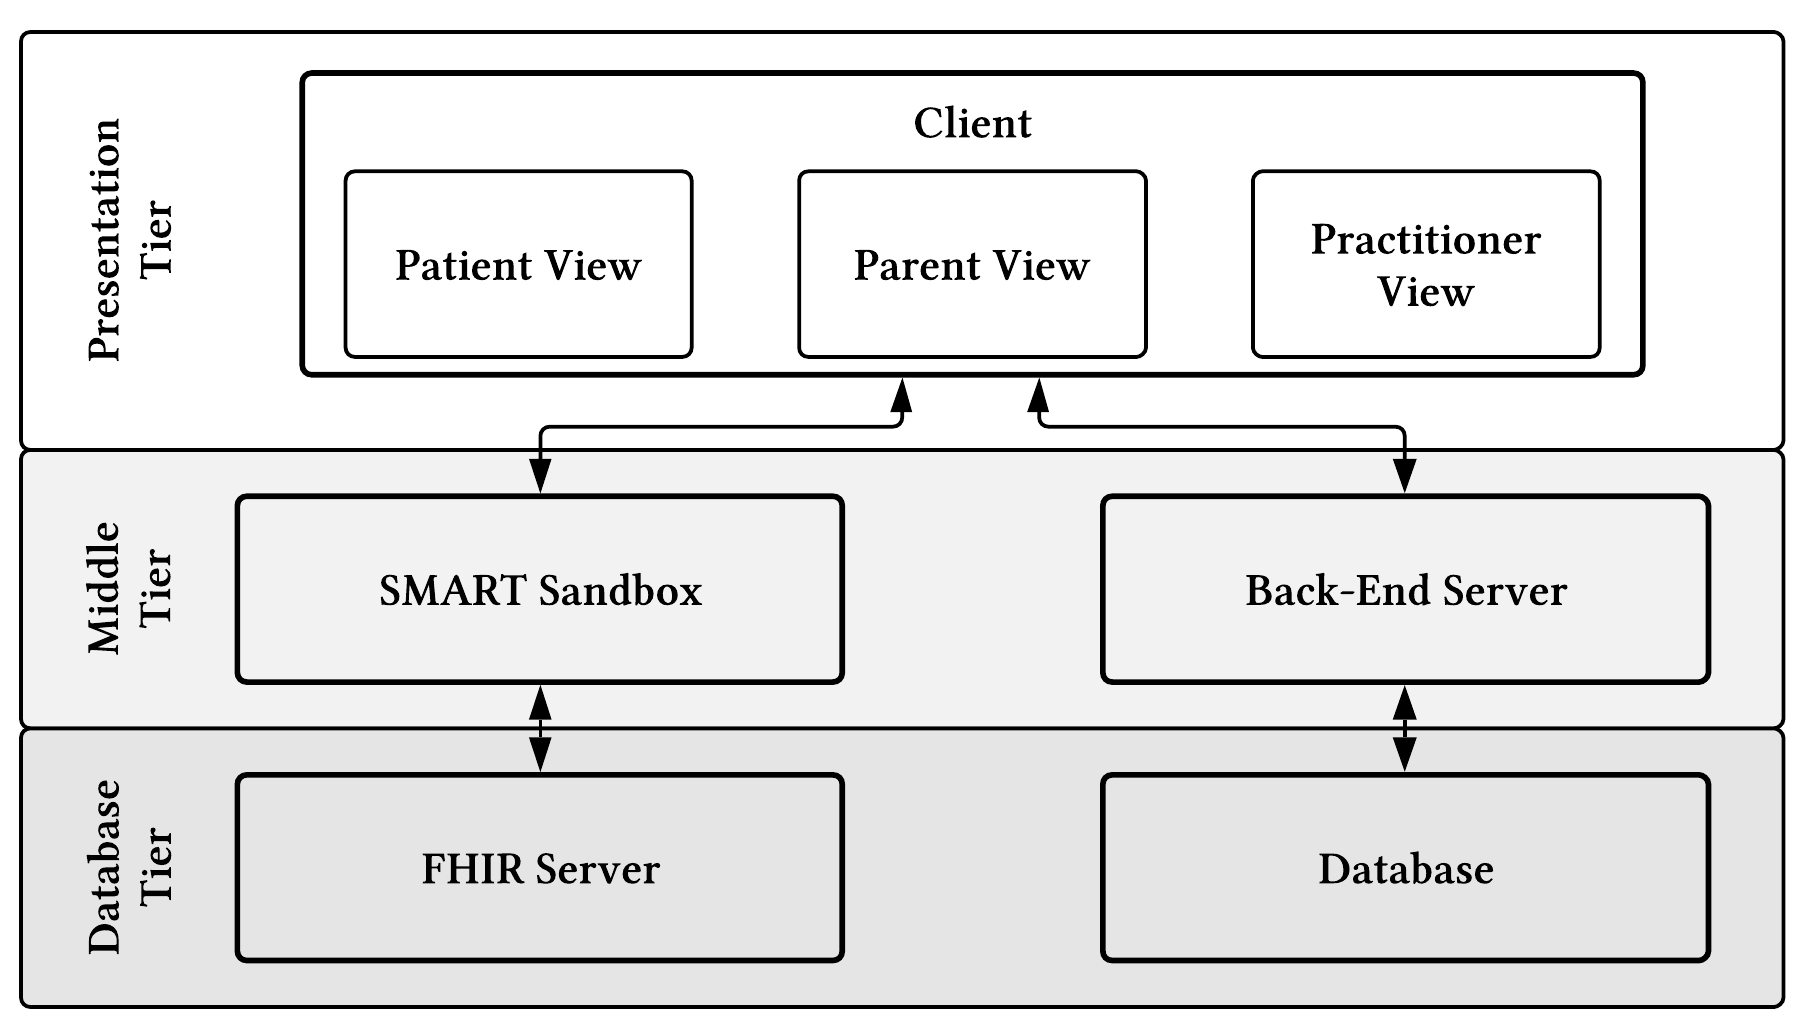
\includegraphics[width=\linewidth]{figures/system_architecture.png}
	\caption{Top-level system architecture diagram displaying Speedy Recovery's three tiers}
	% depicting the Speedy Recovery three-tier architecture}
        \label{fig:system-architecture}
\end{figure}

%\begin{figure}
%	\centering
%	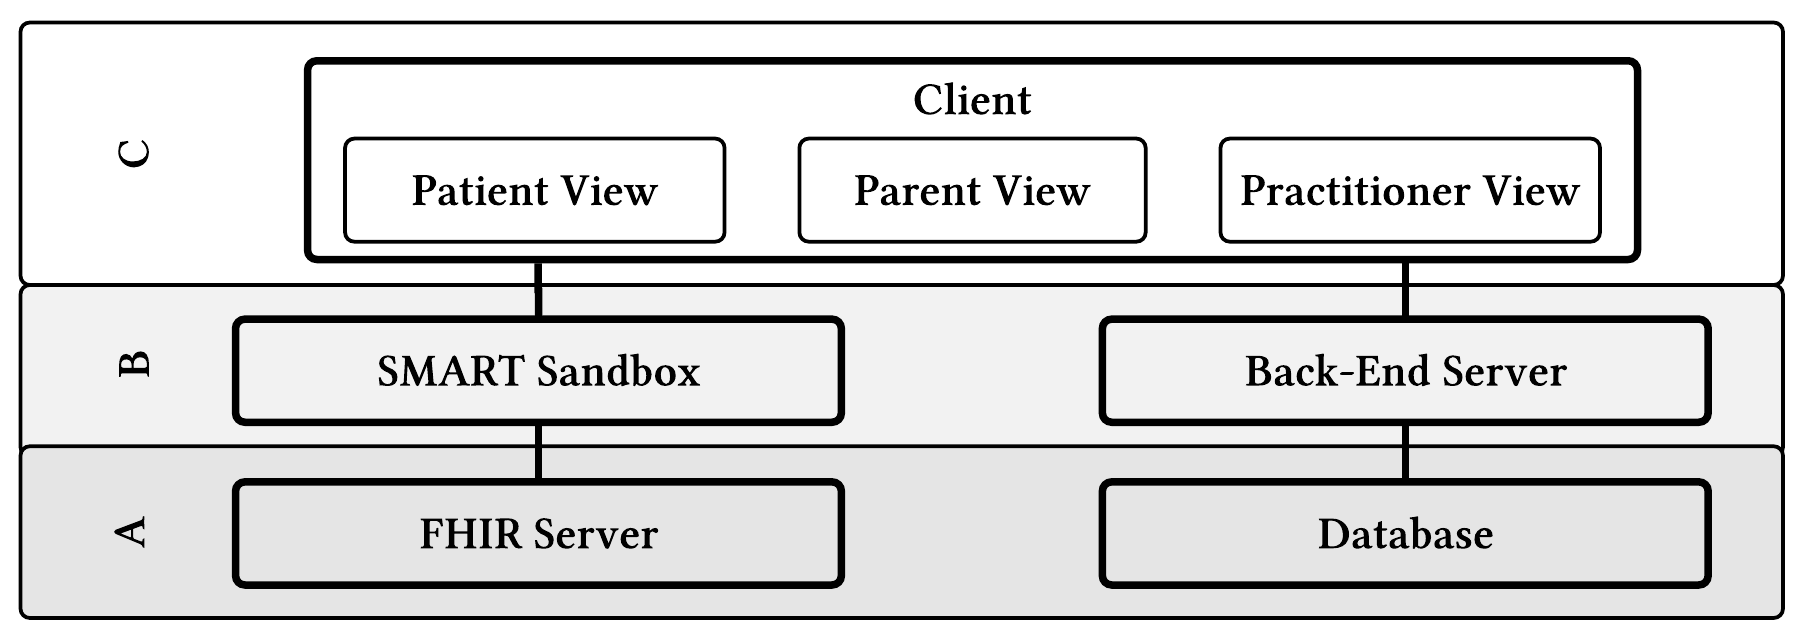
\includegraphics[width=\linewidth]{figures/system_architecture_flat.png}
%	\caption{System architecture diagram showing the A) Database, B) Middle and C) Presentation Tier}
%        \label{fig:system-architecture-flat}
%\end{figure}

In addition to a proprietary back-end and database that have been created specifically for this application, the client interacts with a FHIR server and sandbox, as will be further discussed in the following section.


\subsection{Sub-Components}


\paragraph{Front-End}
\label{sec:front-end}

The core element of SR is in the user-facing web application. From a developer's perspective, it is partitioned into the pages anyone can see and the larger part which can only be accessed upon user authentication. This part displays adjusted content according to the user's role. Both modules are then further broken down into components and sub-components, many of which are parameterised and reused across different role-based views.% The UI components are accompanied by a set of services, which encompass shared business logic (see \ref{sec:modularity}).

The project's package structure reflects this architectural design. In the build process, however, it gets bundled to a small number of static files, which are effectively being served to users when they access the application. As most modern web applications do, SR implements the Single Page Application (SPA) pattern, meaning that all of the HTML, JavaScript and CSS are transmitted at the initial page load, and subsequent interactions only result in exchanges of JSON data, which are usually very small in size. This allows for a quick and responsive user experience, which is known to positively influence user satisfaction~\cite{web-user-satisfaction}~\cite{web-site-usability}. This radical decrease in data traffic compared to older data standards is only made possible through the RESTful structure of FHIR resources~\cite{fhir-official}~\cite{franz2015applying}.


\paragraph{Back-End}

The back-end of our application acts as a level of indirection between the front-end and the proprietary database. Its main functionality is performing simple CRUD operations on the data as requested by the client, and returning data. By routing requests through the back-end rather than accessing the data layer directly, the system can verify and sanitise requests, add additional constraints and business logic according to the user role, and provide logging and monitoring. All interactions go through a set of endpoints which were designed as a RESTful API.

\paragraph{Database}

A simple relational database is installed on the Azure cloud. It is exclusively accessed through the back-end for the reasons mentioned above. The tables reflect the additions made to the FHIR standard in the context of this application, as will be discussed in section \ref{sec:data-architecture}.


\subsection{Role-Based User Interfaces}
\label{sec:rolebasedui}

Building upon our findings from the role-based requirements research (see section~\ref{sec:role-requirements}), we identified user stories for each role and then modified the UI to suit each user.% E.g., the patients' view is the most colourful one, displaying the least amount of data. The practitioners' view, on the other hand, maximises the information displayed and uses a more neutral design.
As the front-end is assembled from nested components, different views effectively render different combinations of components. The implementation details will be discussed in the following sections.
% todo: if we have space
% Adjusted level of depth, abstraction, information
% mention responsiveness; assumption that will run on Ipad, presentation is important


\subsection{Architectural Strategies and Patterns}
\label{sec:strategies-patterns}


\subsubsection{Modularity and Extensibility}
\label{sec:modularity}

As mentioned above, we made sure to reflect our architectural design in the structure of packages, modules and components. Not only does this make for more readable and understandable code, it also allows for the system to be easily maintained and extended in the future. %, e.g. following the release of a new FHIR version.
Clear-cut modularity inherently leads to separation of concerns. As the core application was implemented using React, it is naturally assembled from multiple nested components, thus implementing the composite design pattern~\cite{design-patterns}. These building blocks partition the code-base into distinct parts, which can be tested individually, and mitigate debugging as they prohibit errors propagating uncontrollably.

Alongside these components which correspond to visual elements rendered to the page, we identified shared functionality and business logic (e.g. requesting data from external sources, filtering, or mapping data) and extracted them to semantically related service modules. These modules provide certain well-defined interfaces, which are then imported into and invoked by other components.


\subsubsection{Interoperability and Portability}
\label{sec:interoperability}

Interoperability is a key factor in modern HIT systems. The term refers to effective information sharing between care settings, organisations and geographies, as well as between professionals and citizens~\cite{nhs-interoperability}. This is the main idea behind the FHIR standard. However, as we have already mentioned in section \ref{sec:challenge-integration}, the interfaces of commercial HIT system vendors diverge by a surprisingly high amount. 
%
To mitigate this problem, we made SR discover its run-time environment and implemented support for different settings, thus making the application portable and a deployment to another EHR is thereby feasible and inexpensive. If, for example, GOSH was to deploy the application internally after they migrate to Epic in April 2019, %and provided Epic would permit them a less restrictive interface than their generic systems provide (see section  \ref{sec:ehr}), SR 
it would need little adjustment in order to run in that environment.

When the application is started, the client issues a request for a so-called \texttt{CapabilityStatement} from the FHIR server. The response contains information about, amongst others, the following properties:
the version of FHIR,
the subset of FHIR resources exposed and
for each resource, which operations are permitted.
%
This allows the application to adjust accordingly, as will be discussed in the ensuing sections. In theory, the version could also be hard-coded at the time of deployment, as the server setting should be known at that point. Our implementation, however, has the advantage of dynamically adapting to a different version if the server should change its configuration, with no need to re-deploy the application.

For the time being, the two FHIR versions provided by the SMART sandbox (DSTU2 and STU3) are supported. While the development is mostly based on the more recent STU3 release, the DSTU2 conformity was manually verified and is covered by tests.% a test-suite


\subsubsection{Adaptability}

It is expected that SR is able to adapt to its environment as described above, but in addition to that, the app has to also adapt to the role of the current user. To achieve this, we designed the application to be loosely coupled and leverage the Adapter pattern alongside the Abstract Factory pattern and the Dependency Injection technique~\cite{design-patterns}.
%
All raw FHIR data is passed through a data processing chain made up of multiple service method calls. This design can easily be extended in the future. As of now, it consists of a filtering and a mapping step. The data mapping service uses an adapter, which carries out the mapping to the internal data structure. Depending on the server's \texttt{CapabilityStatement}, a different adapter implementation is chosen at run-time. 

As part of the login process, the user chooses which role they want to login as. Depending on their choice, they get redirected to a different sandbox configuration URL. These URLs, in conjunction with related settings, are stored in distinct configuration files. The correct configuration is injected according to the users' input.

Finally, we make use of the Abstract Factory Pattern to solve the problem of displaying similar, yet different UIs to each role. As we established in \ref{sec:challenge-roles}, this setting could potentially lead to either lots of duplicate code or lots of complex conditionals. We tried to strike a balance by mostly reusing the same components, as well as identifying certain families of components which follow the same structure, but have different concrete manifestations for each role. To generate appropriate sub-components for these groups, we leveraged so-called abstract factories. In the future, more roles could be added without altering the basic structure.


\subsubsection{Resilience and Graceful Degradation}
\label{sec:graceful-deg}

As the previous sections have shown, SR is capable of detecting its  environment's capabilities and adapting accordingly. Certain  properties are optional, allowing the system to still be functional,  with some features being disabled.% (e.g. if the FHIR server grants read-only access to crucial resources).
However, as there are numerous possible constellations of settings and versions, and as the application itself depends on environmental factors outside of its control, the system was built to handle errors gracefully. Erroneous responses, network errors or subsystem outages of the EHR (respectively sandbox), FHIR server, or the SR proprietary back-end and database are expected and will not cause the application to stop working altogether. Instead, an error message is displayed, and depending on the nature and severity of the failure, the user can continue to use the system. An automated test-suite guarantees this behaviour.


\section{System Integration}
\label{sec:system-integration}


\subsection{Deployment}

The proprietary system components, made up of the SR front-end and back-end, are deployed onto the Infrastructure-as-a-Service (IaaS) platform Microsoft Azure. The release pipeline (see \ref{sec:cicd}), transfers the build artefact of the most recent successful build into a container hosted on Azure, where the application is then being served and is accessible at a public URL.


\subsection{EHR Environment}
\label{sec:ehr}

%Unlike applications developed in other domains, applications in HIT, particularly in the context of FHIR, never have complete control over all components of the system, as they are embedded into an information system called EHR. 
As we stated in section \ref{sec:challenge-integration}, HIT applications always run in the context of an EHR. This system offers authorisation, authentication, and context information, for example, which user is currently logged in. Third party applications can then launch either directly inside the EHR's interface %, typically implemented as an HTML \texttt{iframe}, 
or launch as standalone applications, remotely accessing the EHR through a specified interface.%, acting as a facade layer.

As mentioned in section \ref{sec:system-integration}, it was not possible for us to develop against real patient data and deploy to production within GOSH's real infrastructure. %Even if it were not for the privacy issues of patient data, GOSH's IT systems are currently in transit, as they are being prepared for the switch to a new Epic system. As a consequence of this, GOSH could not even offer us any access to their systems or de-identified data in any way. Instead, 
Therefore, we were advised to choose a publicly available sandbox instead. Sandboxes are virtual environments, which act as a proxy for EHR systems. They offer an abstraction of all the core features typically provided by the EHR, and thereby facilitate development and testing. All significant EHR vendors provide their own sandbox, corresponding to the specifications and characteristics of their system. Additionally, a popular sandbox is provided by the creators of the SMART on FHIR specification.% (Boston Children's Hospital Computational Health Informatics Program and the Harvard Medical School Department of Biomedical Informatics).

Initially, our efforts were focused on the Epic sandbox, as this environment would have been the one most closely aligned to the EHR our client will install in the near future. However, we were faced with a succession of severe drawbacks.
% \begin{itemize}
%     \item Setting up a new application is tedious and requires the developer to answer a lot of % questions on the usage and scope of the product which might not be decided on at an early stage % of the project. Also, it requires secure links to publicly provided resources such as system % documentation, terms and conditions, etc.
%     \item Some features and the better part of the documentation are not publicly accessible. % Developers first have to request an account for the Epic App Orchard subsystem, a process that % according to Epic takes 2--3 weeks.
%     \item Epic systems, and accordingly the sandbox, provide a very constrained FHIR interface to % their internal data\footnote{https://open.epic.com/Interface/FHIR}:
%     \begin{itemize}
%         \item The most recent supported version is the outdated DSTU2.
%         \item The interface is limited to read-only access.
%         \item The interface is restricted to a small subset of all available FHIR resources.
%     \end{itemize}
% \end{itemize}
% 
After having already spent a significant amount of time %setting up the Epic sandbox and designing the API calls
, it became more and more obvious that we would not be able to satisfy our system's requirements in this setting. The deciding factor, in the end, was the fact that the \texttt{Appointment} resource, a central entity for implementing a calendar, was excluded from Epic's interface. Therefore, we had to abandon this sandbox. % at a relatively late stage, which set us back and challenged our planned schedule.
%
We then shifted to the SMART on FHIR sandbox, %which does not have any overhead at all when creating a new application. 
which offers a much less restrictive interface. %Anyone can access its launch page, configure a specific environment for an application, and access it through a generated unique URL. 
Also, it provides read and write access to the complete FHIR specification in both the DSTU2 and STU3 versions.


\subsection{Authorisation and Authentication}
\label{sec:auth}

The FHIR specification itself does not have a concept of security and access control. However, the SMART on FHIR platform, which includes guidelines for authorisation and authentication in its Application Launch Framework, provides a widely adopted de-facto standard and leverages contemporary web standards like RESTful APIs~\cite{smart-on-fhir}. 
%On top of that, it obviously cooperates very well with the SMART sandbox, being developed by the same organisations. 
Given that we operate under the assumption that SR runs inside an environment that has already authenticated its user, the system needs a way of accessing user information and verifying the user's identity. By implementing the SMART App Launch Framework protocol, SR authorises and authenticates users with the common web standards OAuth 2.0 and OpenID~\cite{smart-launch-framework}. As part of the login process, users implicitly request access to clinical data scopes. For standalone SMART apps like ours, the browser redirects the user to the EHR/sandbox UI, where the login itself takes place. Then, the browser again redirects back to the application, while also sending a secure payload containing the authentication response.


\subsection{FHIR Data Server}

The FHIR data server is a crucial part and the main data source for SR. For development and testing, the server provided through the SMART sandbox was used in different configurations, including the DSTU2 and STU3 FHIR versions together with several combinations of access privileges.


\section{Data Architecture}
\label{sec:data-architecture}

\paragraph{Data Flow}

The main source of information for SR is a set of resources retrieved from FHIR, including \texttt{Patient}, \texttt{Practitioner}, \texttt{RelatedPerson}, and \texttt{Appointment}, among others. Unlike older standards, the RESTful approach of FHIR data allows for fine-grained access and heavily reduces data traffic~\cite{franz2015applying}. This data then gets combined with the proprietary extensions and passed through a data processing chain, which filters invalid data and transforms the various input formats into a coherent, internal data structure. As of the limitations of GOSH's infrastructure (see section \ref{sec:challenge-integration}), currently FHIR-based data access is read only.

Within the client, data flows down the component hierarchy. Following the suggested React architecture~\cite{react-lifting-state}, state which multiple components access is maintained by the closest common ancestor.
%todo: if we have space, mention some assumptions in data model (like only 1 child, ..)


\paragraph{Data Extensions}

One of the general limitations of the FHIR standard is that it cannot be adjusted or extended~\cite{fhir-official}. As the context of SR benefited from certain additional pieces of information, we extended the data model by joining the FHIR data with information stored in a distinct database, for example, to add personal details about clinical staff. This proprietary server also grants  write-access, enabling, for example, the messaging feature to be implemented.


\paragraph{Data Generation}

As the synthetic patient data provided by the SMART on FHIR data server turned out to be sparse, especially regarding patients in childhood, we generated some additional data tailored to test SR. As the server gets reset on a nightly basis, we wrote an idempotent data generation script which is designed to guarantee reproducibility and consistency, while also keeping a log of each created resource. In addition, we created the aforementioned data extensions on the proprietary server.


\section{Software Development Tools and Techniques}
\label{sec:tools-and-techniques}


\subsection{Languages, Libraries and Frameworks}
\label{sec:languages}

Early on, we decided to build a web-based application rather than a native one, as this promised the highest reach. % given that the application would be accessible from a broad range of devices. 
The choice of appropriate tools was to a large degree informed by our prior experiences paired with current results of the annual large-scale survey "The State of JavaScript"~\cite{state-of-js}. We chose to build SR using React%as the main client library, 
, as it clearly dominates the survey. As a consequence, the application was mostly written in JSX, with some bits of traditional HTML, JavaScript (JS) and CSS. For styling purposes, the Semantic UI library was incorporated. For the back-end, Node.js was used.

For the JS parts, we utilised many features from the modern ES6 standard, such as arrow function expressions for compact and readable code, or JS modules, allowing us to structure the code in a way that reflects its semantic composition.
% this is kinda verbose and could be cut down if need be

The dependency management tool yarn was used not only to keep track of dependencies, but also to run the development server, the test-suites, and the build process. Within its workflow, we integrated multiple tools from the JS ecosystem, for example, the code style checker ESLint and the code formatter Prettier. %, the latter of which is run as a pre-commit hook to ensure consistent code formatting. 
The build process also minifies and bundles the code, before transpiling it to a broadly supported JS version. In addition, it adds polyfills for modern and experimental features to increase backward compatibility with older browsers and provides cross-browser compatibility.% The build artefact comprises a directory of static HTML, JS and CSS files.

In terms of domain-specific third party libraries, SR makes use of the FHIR JS client maintained by SMART. We also evaluated fhir\=/smartr, a React-specific library that acts as a wrapper around the aforementioned JS client, but abandoned it as it didn't fit our design choices % (as we aim to outsource data access from React components to plain JS service modules).
(using plain JS service modules for business logic).

For testing purposes, we implemented a stack which is typical for React development, with Jest as the main test framework, offering a large set of assertions and matchers, accompanied by Enzyme.% and Mocha.
%, which provides many useful utilities. Additionally, Mocha was used in the back-end.%To test Node.js, we used Mocha.js.


\subsection{Testing and Validation}
\label{sec:testing}

Using the testing setup described above, we strove to consistently maintain a statement coverage of 80\% or above. Our tests comprise a multi-layer testing strategy %Depending on how critical components or services are, we cover them with smoke tests, unit tests, snapshot or integration tests. 
, and the complete test-suite automatically runs on every commit, thus preventing regressions.


\paragraph{Smoke Testing}

Simple smoke tests were written for every component that renders to a visual DOM element. %These tests are very cheap to write and run; the component is merely mounted to an in-memory representation of the DOM. Smoke tests 
While they only provide limited confidence, they do allow us to detect failures quickly.


\paragraph{Unit Testing}

For more complex components as well as service modules, traditional unit tests were written. Often, we made use of shallow rendering in order to ignore nested sub-components and test components in isolation. Also, we made heavy use of the mocking features offered by Enzyme, mocking not only external requests, but also deeply embedded HTML5 browser APIs like \texttt{fetch()} and \texttt{sessionStorage}.% In place of responses from external systems, the tests use static JSON files that were either intercepted from real server transactions or hand-crafted.


\paragraph{Snapshot Testing}

Snapshot tests were mostly implemented for components which we expect to remain stable and want to guarantee a well-defined API. At the time of writing, this mostly comprises the elements of the data processing chain.%, i.e. the services that conduct the filtering and mapping of FHIR data. 


\paragraph{Integration Testing}

As we have pointed out, system integration is a crucial aspect of this project. Therefore, we implemented several integration tests which cover the interactions with the sandbox and the FHIR server. %These tests also make use of a special feature that the sandbox provides: when using particular URLs, a range of authentication errors are simulated. 
We used intentionally erroneous sandbox settings to improve error handling (see section \ref{sec:graceful-deg}) in a test-driven approach. Similarly, we test the system against a set of pre-constructed \texttt{CapabilityStatements}, which are both valid and invalid.


\subsection{Collaboration and Version Control}
\label{sec:version-control}

As a development team, we worked on a shared Git repository and applied Vincent Driessen's Gitflow branching model, as it is known to facilitate collaboration and scaling of the team capability~\cite{git-flow}. Team members or sub-teams worked on dedicated feature branches. As a feature was completed, it got merged back into the development branch. Only when we deployed to production did we merge the development branch back to master.

In order to guarantee a high code quality standard, we implemented a quality gate process by requiring each merge to be approved by at least one code reviewer. This often lead to extensive discussions and many additional changes being added.


\subsection{Continuous Integration and Deployment}
\label{sec:cicd}

From an early stage, we installed build and release pipelines on Azure DevOps and registered them with the SR repository. Both pipelines can be triggered manually, and additionally trigger under given circumstances.

The \textit{build pipeline} triggers at every commit on every branch, and consequently runs the tests and builds the artefacts. Accordingly, the team gets notified immediately when build failures occur or a test case fails.

To enable the aforementioned strategy for branching and deployment, the \textit{release pipeline} triggers whenever commits are being merged into the master branch.


\subsection{Agile Practices and Project Management}
\label{sec:agile}

We loosely followed a Scrum-based workflow, structuring our schedule into multiple sprints, in which we first created a basic prototype, and subsequently enhanced it in each iteration. We also broke down our workload into features, user stories, and tasks, which would then be assigned to individual team members or sub-teams to work on them independently. For critical user stories and tasks, we defined acceptance criteria. % When all the stories comprising a feature were completed, it corresponded to the achievement of a milestone.
%
Every 1--2 weeks, we met in person to have a retrospective and do the planning for the following iteration. At about the same rate, we also met with our clients face-to-face to clarify questions and present our progress.

To manage our backlog, plan iterations, and keep track of the progress on a virtual taskboard, we utilised Azure DevOps Boards. Each feature, user story, and task respectively translated to a digital work item, onto which descriptions and discussions could be added. Additionally, we used the included Wiki feature to document key decisions and findings.% For both internal and external communication, we employed Slack. In order to not clutter the main channels, multiple topic-based sub-channels were created.


\section{Evaluation}
\label{sec:evaluation}


Approaching the end of the development phase, we attempted to evaluate our achievements and the code-base at hand. We performed a qualitative evaluation following the framework suggested by~\cite{evaluate-codebase}. We slightly adjusted the dimensions of the framework insofar as we added two additional assessment criteria to provide a more comprehensive overall impression: testability, as proposed by~\cite{evaluate-criteria}, and architecture quality, as proposed by~\cite{evaluate-achitecture}.


\paragraph{Readability}

Knowing that our finished product would be open sourced and potentially built upon in the future, we always strove to write readable, clean code. First, we agreed on a naming convention for all elements, ensuring semantic naming and descriptive code. Where we found ourselves writing in-line comments explaining our logic, we instead simplified and renamed to convey the meaning. As mentioned in section \ref{sec:version-control}, we used pull requests to conduct code reviews and didn't merge any line of code without approving it.

To help ensure compliance with coding style conventions we incorporated ESLint into our automated build process, which analyses the code for any violations and, if appropriate, causes the build to fail. Similarly, we included Prettier, which in the form of a pre-commit hook automatically re-formats changes before they are committed to the repository (see section \ref{sec:languages}). We are therefore confident that the code-base is readable and complies with common style practices.


\paragraph{Adaptability}

Throughout the project we have employed several different techniques to make the application easily adaptable in the future. The strategies and patterns discussed in section \ref{sec:strategies-patterns} allow one to easily add new pages, features or user roles, as the code-base follows a modular design and the business logic is dynamic. Design choices including the Adapter pattern, the Abstract Factory pattern and Dependency Injection guarantee a loose coupling.


\paragraph{Maintainability}

The aforementioned modularity of our code as well as the effort we spent to produce readable code also increase its maintainability. What's more, the build and deploy workflow we established in section \ref{sec:cicd} makes it easy to verify that future changes will not break the build. Also, it makes deploying a new version to production very easy to carry out.

While SR is built to be resilient and dynamically handles server failures and authentication problems, we have not implemented a way for the application to recover from errors, issues or outages on its own without developer intervention.


\paragraph{Performance}

Throughout our development, we used Chrome DevTools for profiling and detecting performance issues with specific components~\cite{react-profiling}. Before pushing to production, the build pipeline minifies and optimises the code, as discussed in section \ref{sec:languages}. As the SR client is a SPA, the first page load is relatively slow (around 1.6 seconds), while every subsequent transaction will only transfer minimal amounts of data, allowing for a fluent user experience.

While we did manually verify that SR reacts promptly to user input, we have not conducted any formal, or even automated performance tests yet. Also, the caching only goes as far as the browser is able to automatically carry it out. We do not currently use any advanced caching mechanisms like Service Workers.


\paragraph{Accuracy}

Accuracy is crucial for any app that displays medical information to its users, and is fundamental for trustworthiness. This is a key success factor of healthcare applications~\cite{trustworthy-apps}. Our main source of data is a FHIR server, which provides the core resources that SR processes. Therefore, we are in a way delegating the responsibility for accurate data to the clinical environment. For the additional data we introduced to extend the FHIR standard, the same implications apply: our system, to a large degree, depends on the environment to ensure the accuracy of the data. This is due to SR at its core providing the view layer for existing clinical data. However, we implemented a data filtering layer that removes obviously incomplete or invalid data to mitigate the problem and increase confidence in our system.


\paragraph{Security and Privacy Protection}

The danger of compromises in patient confidentiality is one of the most important problems in HIT~\cite{lack-of-evidence}. As discussed in section \ref{sec:ehr}, we are implementing the security specifications as defined by SMART on FHIR, meaning that users are authorised and authenticated through a combination of OpenID and OAuth 2.0. All transactions are carried out using the SSL protocol. As the authentication as well as critical information are retrieved directly from the EHR (respectively the sandbox), the code running on the client's device can assume them to be sound.

However, the current version of SR is only deployed against the SMART sandbox, inside a test environment. For a real-world deployment, it would be necessary to consult IT security experts and empirically prove the security of the system. What's more, our proprietary back-end is currently using an unprotected connection.


\paragraph{Interoperability}

As we have extensively discussed in section \ref{sec:interoperability}, interoperability was one of the key aspects we considered when developing SR. It is built on the FHIR data model, which in turn is founded on the ideal of enabling interoperability between health systems. We also implement the SMART on FHIR specification, thus further enhancing the portability of our app. While the FHIR standard is still evolving and the concrete implementations of EHR vendors vary, we developed several means of delivering interoperability, as discussed in \ref{sec:strategies-patterns}.


\paragraph{Usability}

Founded on the research carried out in section \ref{sec:role-requirements}, we designed each view to be optimised for one specific role. For example, the patient view was designed to be very colourful and include lots of pictures that would make it much easier for a child to use. In contrast, the practitioner and parent views are much more data focused, seeming as their priority is to display information about the patient and their treatments. 

In order to quantitatively measure and improve the usability or SR, it would be useful to carry out user testing and gather feedback from the actual users of the app, rather than just our clients at GOSH. A particular area of interest would be to improve accessibility, as users in the HIT context are potentially more likely to be impaired. Additionally, adhering to the commonly agreed Web Content Accessibility Guidelines (WCAG) by the W3C, could make the app more child friendly.


\paragraph{Software Engineering Process}

We found the software engineering processes and techniques we described in \ref{sec:languages} to help us work as a team very efficiently. The agile, iterative approach helped us to have early successes and steadily reach our milestones. For example, we finished the first prototype after two weeks and had the first version running in production after five weeks.

The Gitflow branching strategy allowed us to work on the project in parallel, while the code reviews before each merged helped ensure high code quality. Our continuous communication through digital channels was enhanced with weekly face-to-face meetings and the product quality certainly benefited from gathering client feedback early and often.

While we occasionally used pair programming, this could have been done more often, as we were sometimes challenged to have all team members share the same level of knowledge. Also, there were a few cases of miscommunication, resulting in two developers solving the same problem.


\paragraph{Testability}

As we discussed in section \ref{sec:testing}, we put great effort into devising a comprehensive testing strategy. Starting from well-defined, fine-grained components that could easily be tested in isolation, we wrote different types of tests as appropriate. We aimed to maintain a statement coverage of at least 80\%, and ran the tests at every push to the repository.

At the time of writing, our code-base is covered by 37 test-suites, comprising 218 test cases and 16 snapshots, and providing 83.68\% statement coverage 91.91\% branch coverage. However, there is still room for improvement, as we, for example, do not perform load testing, performance testing, or click-driven UI testing.


\paragraph{Architecture Quality}

The 3-tier architecture structure is a traditional and proven design for web applications. It provides portability between cloud platforms and on-premises deployment, is widely known amongst developers and provides a natural evolution from the traditional application model. There are, however, some trade-offs. The middle tier often just implements basic CRUD operations on the database, adding extra latency without doing a lot of useful work. This can lead to monolithic designs, as the layers typically depend on each other, rendering an independent deployment of features impossible. We follow some best practices, for example, using asynchronous messaging to decouple tiers. However, we could significantly improve scalability and resilience if we implemented auto-scaling (potentially including containerised deployment) and high availability for the data tier.~\cite{ms-ntier}. Research has shown that the potential scalability benefits of cloud computing can improve HIT applications significantly~\cite{cloud-computing}.

Within the sub-systems, like the front-end, we have implemented architectural strategies and patterns to make them maintainable, extensible, portable and adjustable (see section \ref{sec:strategies-patterns}).


\section{Future Work}
\label{sec:future-work}


\subsection{Integration into Internal Infrastructure}
At the moment, SR is using the SMART sandbox together with a temporary back-end server in order to retrieve its required data. In order to actually deploy our app in a hospital, we would have to integrate it into the hospitals' internal infrastructure. First, we would have to switch to GOSH's FHIR server instead of the one provided within the SMART sandbox. This would mean for our app to process real patient data, which would also imply much higher security standards to be satisfied, due to the sensitive nature of health-related information. The app would presumably be restricted to run within the hospital's secure network and all users would have to go through an enabling process, in which their identity is verified by the hospital. The actual migration wouldn't require many code changes however, as we outlined in section \ref{sec:interoperability}.

During development, we assumed that we did not have the rights to write data to FHIR due to the restrictions of Epic's API. However, if the app would be integrated into the hospitals internal systems, we might gain this functionality, and could, for example, enable users to create or request new appointments from within SR. This would be a very useful feature for parents, who currently have to contact hospital staff directly to make new appointments.


\subsection{Other Areas of Improvement}

In addition to the system integration and improving on the limitations that were discussed in section \ref{sec:evaluation}, there are some other areas which might be of interest for future developers to work on:

\begin{itemize}
    %\item Add functionality to allow our app to interface with other systems and the outside world.
    \item Adding more features to further distinguish the three views.
    \item Analysing potential security and privacy issues and adding countermeasures, especially for the proprietary back-end.
    \item Improving non-functional requirements such as accessibility.
    \item Conducting extensive user testing and improve role-based UIs based on feedback.
    %\item Think about how our app can be further extended by the NHS.
    \item Improving scalability by creating a containerised deployment and setting up auto-scaling.
    %\item Improving the availability of the application.
    \item Creating a platform-specific native app from the code-base.%version of our app allowing for improved usability on mobile devices.
\end{itemize}


\section{Conclusion}
\label{sec:conclusion}

The use of electronic devices and digital applications is becoming an increasingly important component of healthcare. Some well-known shortcomings of older data standards need to be overcome in order to provide more effective information sharing between systems and organisations, as well as between patients and healthcare providers. The FHIR standard was conceived in the hope of delivering this improved interoperability, and together with the SMART on FHIR specifications, it is increasingly being implemented and supported by EHR vendors.

In this project, we collaborated with GOSH and applied these technologies to solve a real-world problem. We created a web-based application tailored to facilitate the day-to-day tasks of paediatric patients, their parents and healthcare providers. In order to account for the different requirements, we developed an application architecture that adjusts its properties and functionalities to each role while supporting portability between different healthcare systems.

The main challenges we faced were role-based access, system integration and inconsistent data. We approached these by developing a modular, loosely coupled, adaptive architecture that supports graceful degradation. Eventually, we successfully delivered a functional application for our client GOSH to use and build upon. Our results can potentially be the basis for other projects in the HIT context and we hope to thereby improve the quality of care and the overall patient experience in the long term.


\newpage


%
% The next two lines define the bibliography style to be used, and the bibliography file.
\bibliographystyle{ACM-Reference-Format}
\bibliography{references}


\end{document}
